%#################### 9.1 ####################
\subsection{\hll{LaTeX Coffee Stains}}
\begin{table}[h!]
\begin{tabular}{c | c}
\begin{minipage}[m]{0.4\textwidth}
\enum{\cofeAm{1}{0.6}{0}{0.cm}{6.5cm} 

\cofeCm{0.9}{0.5}{180}{-7.cm}{11cm}

Download \fbox{coffee4.sty} and put in the same directory

\cofeDm{0.2}{0.2}{90}{0.5cm}{2.5cm}
\cofeBm{0.5}{0.5}{0}{-3.cm}{10cm}

 }{\href{https://www.overleaf.com/latex/examples/latex-coffee-stains/qsjjwwsrmwnc}{9.1}}

\end{minipage}
&
\begin{minipage}[m]{0.55\textwidth}
\renewcommand\textminus{\mbox{-}}%<<<<<<<<<<<

\begin{lstlisting}[numberstyle=\zebra{orange!15}{red!15},numbers=left,basicstyle=\ttfamily\footnotesize]
\documentclass{article}
\usepackage{tikz}
\usetikzlibrary{arrows,shapes}
\usepackage{coffee4}
\enum{\cofeAm{1}{0.6}{0}{0.cm}{6cm} 
\cofeCm{0.9}{0.5}{180}{-7.cm}{11cm}
\cofeDm{0.4}{0.2}{90}{1.0cm}{3.0cm}
\cofeBm{0.5}{0.5}{0}{-3.cm}{10cm}
%\cofeAm{alpha}{scale}{angle}{xoff}{yoff} <-- usage
\end{document}
\end{lstlisting}
\end{minipage}
\end{tabular}
\end{table}
%#################### 9.2 ####################
\subsection{\hll{Sticky notes}}
\begin{table}[h!]
\begin{tabular}{c | c}
\begin{minipage}[m]{0.4\textwidth}
\enum{ \href{https://tex.stackexchange.com/questions/26846/how-to-scale-a-tikzpicture-including-texts}{\img{1}{9.3}}}{9.2}

\end{minipage}
&
\begin{minipage}[m]{0.55\textwidth}
\renewcommand\textminus{\mbox{-}}%<<<<<<<<<<<
\begin{lstlisting}[numberstyle=\zebra{orange!15}{red!15},numbers=left,basicstyle=\ttfamily\scriptsize]
\documentclass{article}
\usepackage{xparse}
\usepackage{fancypar}
\usetikzlibrary{calc,shadows}
\NewDocumentCommand\StickyNoteP{O{6cm}mO{6cm}}{%
\begin{tikzpicture}
\node[
drop shadow={shadow xshift=3pt,},
inner xsep=0pt,
xslant=-0.1,yslant=0.1,
inner ysep=0pt,
text depth=\the\dimexpr#1+2.5ex\relax
] {\parbox[t][#1][c]{#3}{#2}};
\end{tikzpicture}}

\begin{document}
\StickyNoteP[2.5cm]{%
\NotebookPar[spiral=false]{
\LARGE first\\  second }}[6.5cm]
\end{document}
\end{lstlisting}
\end{minipage}
\end{tabular}
\end{table}
\clearpage
%#################### 9.3 ####################
\subsection{\hll{\fadingtext[scale=1, font=\bfseries]{path picture shading=rainbow}{Rainbow text}}}
\begin{table}[h!]
\begin{tabular}{c | c}
\begin{minipage}[m]{0.4\textwidth}
\enum{ \fadingtext[scale=2, font=\bfseries]{upper left=red, upper right=green, lower left=blue,lower right=yellow}{\LaTeX} \fadingtext[scale=2, font=\bfseries]{path picture shading=rainbow}{\LaTeX} \\

\noindent\fadingtext[scale=0.7, font=\bfseries]{path picture shading=rainbow}{\parbox[b]{1.5\linewidth}{\strut\lipsum[1]}}

 }{\href{https://tex.stackexchange.com/questions/344260/rainbow-colored-one-letter-with-tikz-and-xcolor}{9.3}}

\end{minipage}
&
\begin{minipage}[m]{0.55\textwidth}
\renewcommand\textminus{\mbox{-}}%<<<<<<<<<<<
\begin{lstlisting}[numberstyle=\zebra{orange!15}{red!15},numbers=left,basicstyle=\ttfamily\scriptsize]
  \documentclass{article} 
  \usepackage{tikz}
  \usetikzlibrary{fadings, shadings}
  \newcounter{fadcnt}\setcounter{fadcnt}{0}
  \newcommand\fadingtext[3][]{%
  \stepcounter{fadcnt}
    \begin{tikzfadingfrompicture}[name=fading letter\thefadcnt]
      \node[text=transparent!0,inner xsep=0pt,outer xsep=0pt,#1] {#3};
    \end{tikzfadingfrompicture}%
    \begin{tikzpicture}[baseline=(textnode.base)]
      \node[inner sep=0pt,outer sep=0pt,#1](textnode){\phantom{#3}}; 
      \shade[path fading=fading letter\thefadcnt,#2,fit fading=false]
      (textnode.south west) rectangle (textnode.north east);% 
    \end{tikzpicture}% 
  }
  \usetikzlibrary{calc}
  \newbox\shbox
  \tikzset{%
    path picture shading/.style={%
    path picture={%
  %
  \pgfpointdiff{\pgfpointanchor{path picture bounding box}{south west}}%
    {\pgfpointanchor{path picture bounding box}{north east}}%
  \pgfgetlastxy\pathwidth\pathheight%
  \pgfinterruptpicture%
     \global\setbox\shbox=\hbox{\pgfuseshading{#1}}%
   \endpgfinterruptpicture%
  \pgftransformshift{\pgfpointanchor{path picture bounding box}{center}}%
  \pgftransformxscale{\pathwidth/(\wd\shbox)}%
  \pgftransformyscale{\pathheight/(\ht\shbox)}% \dp will (should) be 0pt
  \pgftext{\box\shbox}%
  %
      }
    }
  }
  \pgfdeclarehorizontalshading{rainbow}{10bp}{color(0bp)=(violet);
              color(1.6667bp)=(blue);
              color(3.3333bp)=(cyan);
              color(5bp)=(green);
              color(6.6667bp)=(yellow);
              color(8.3333bp)=(orange);
              color(10bp)=(red)}
  \begin{document} 
   \fadingtext[scale=10, font=\bfseries]{upper left=red, upper right=green, lower left=blue,lower right=yellow}{\LaTeX}

  \fadingtext[scale=10, font=\bfseries]{path picture shading=rainbow}{\LaTeX}

  \noindent\fadingtext[scale=0.7, font=\bfseries]{path picture shading=rainbow}{\parbox[b]{1.5\linewidth}{\strut\lipsum[1]}}
  \end{document}
\end{lstlisting}
\end{minipage}
\end{tabular}
\end{table}
\clearpage

%#################### 9.4 ####################
\subsection{\hll{Single Watermark}}
\begin{table}[h!]
\begin{tabular}{c | c}
\begin{minipage}[m]{0.4\textwidth}
\enum{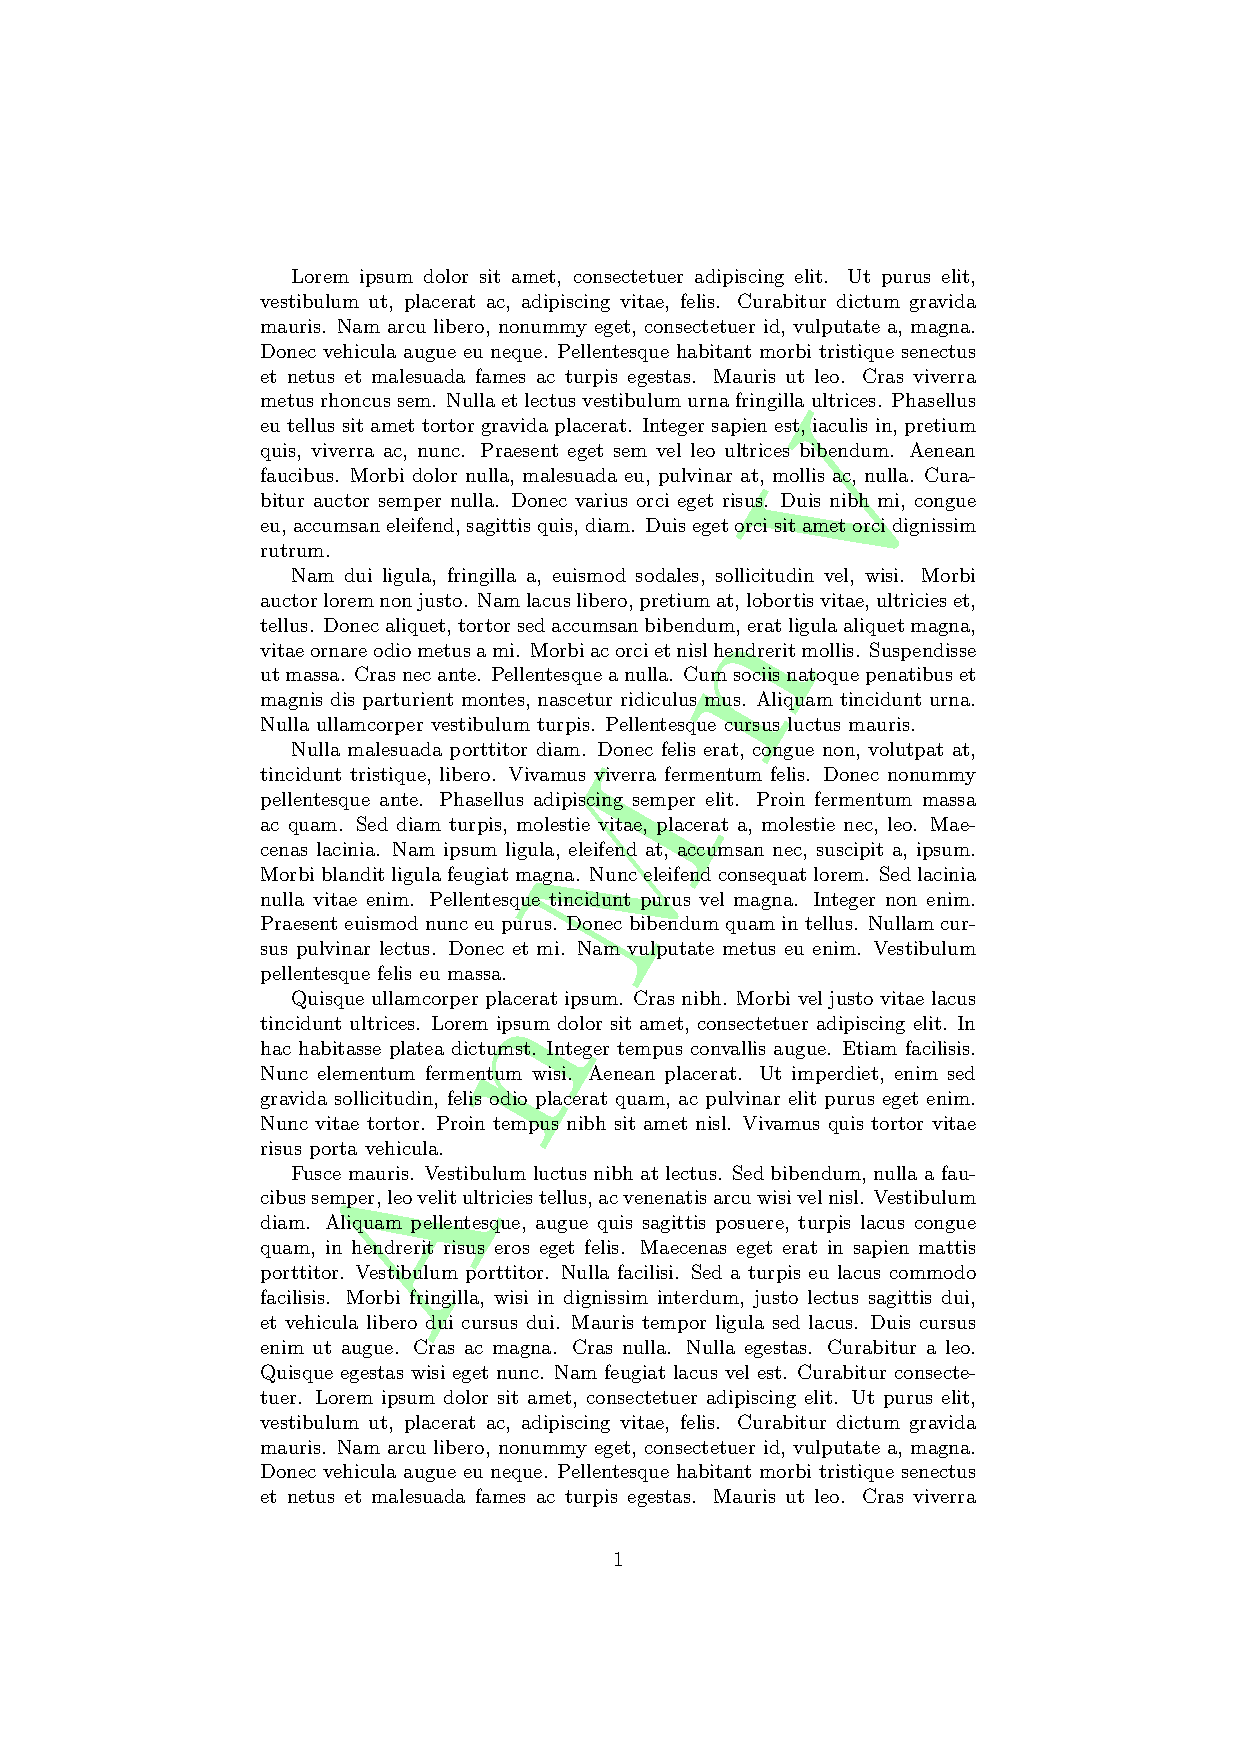
\includegraphics[width=0.9\linewidth]{images/9.4/9.4.pdf}}{9.4}

\end{minipage}
&
\begin{minipage}[m]{0.55\textwidth}
\renewcommand\textminus{\mbox{-}}%<<<<<<<<<<<
\begin{lstlisting}[numberstyle=\zebra{orange!15}{red!15},numbers=left,basicstyle=\ttfamily\scriptsize]
\documentclass[a4paper]{article}
\usepackage[T1]{fontenc}
\usepackage[utf8]{inputenc}
\usepackage[pages=some]{background}% change "some" to "all" to see WM on all pages 
\usepackage{lipsum}
\backgroundsetup{color=green, opacity=0.3, scale=10, contents={A n M n V}}

\begin{document}
\lipsum[1-5] 
\BgThispage
\lipsum[1-5]
\end{document}
\end{lstlisting}
\end{minipage}
\end{tabular}
\end{table}
%#################### 9.5 #################### 
\subsection{\hll{Full page of Watermarks}}
\begin{table}[h!]
\begin{tabular}{c | c}
\begin{minipage}[m]{0.4\textwidth}
\enum{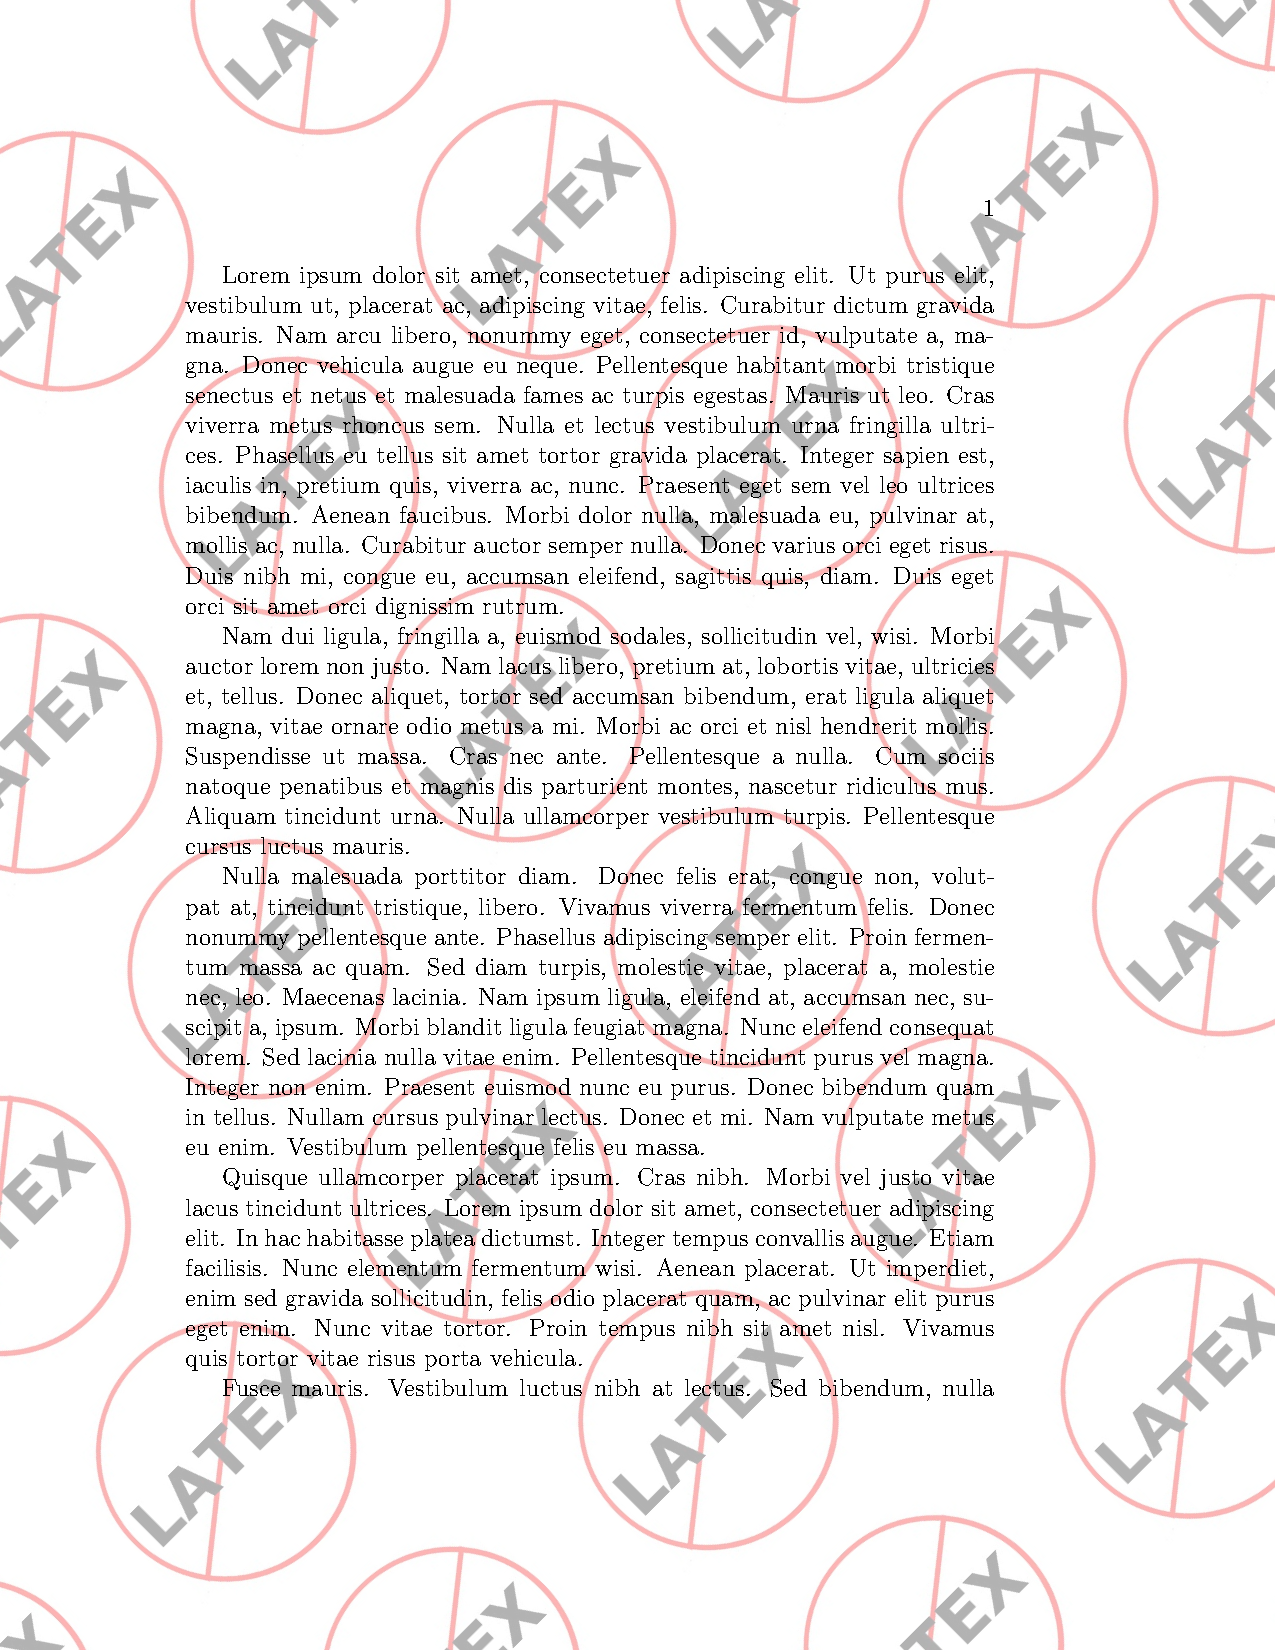
\includegraphics[width=0.9\linewidth]{images/9.5/9.5.pdf}}{9.5}

\end{minipage}
&
\begin{minipage}[m]{0.55\textwidth}
\renewcommand\textminus{\mbox{-}}%<<<<<<<<<<<
\begin{lstlisting}[numberstyle=\zebra{orange!15}{red!15},numbers=left,basicstyle=\ttfamily\scriptsize]
\documentclass[12pt]{book}
\usepackage{graphicx}
\usepackage[pages=some]{background}
\usepackage{lipsum}
\newcommand\DupImage{%
     
\includegraphics[width=5cm]{logo.jpeg}\hfill%  YOUR IMAGE
     
\includegraphics[width=5cm]{logo.jpeg}\hfill%  YOUR IMAGE
     
\includegraphics[width=5cm]{logo.jpeg}\hfill%  YOUR IMAGE
     
\includegraphics[width=5cm]{logo.jpeg}\hfill%  YOUR IMAGE
     
\includegraphics[width=5cm]{logo.jpeg}\hfill%  YOUR IMAGE
     
\includegraphics[width=5cm]{logo.jpeg}\hfill%  YOUR IMAGE
     
\includegraphics[width=5cm]{logo.jpeg}\hfill}
\newlength{\drop}
\backgroundsetup{  scale=1, angle=45, opacity=.3, 
  contents={%
     \begin{minipage}{1.5\paperheight}
     \DupImage\\[2ex]
     \DupImage\\[2ex]
     \DupImage\\[2ex]
     \DupImage\\[2ex]
     \DupImage\\[2ex]
     \DupImage\\[2ex]
     \DupImage\\[2ex]
     \DupImage\\[2ex]
     \DupImage\\[2ex]
     \DupImage  \end{minipage}   }  }

\begin{document}
\drop=0.1\textheight \BgThispage \lipsum[1-8]
\end{document}
\end{lstlisting}
\end{minipage}
\end{tabular}
\end{table}

%#################### 9.6 ####################
\subsection{\hll{Generating QR code}}
\begin{table}[h!]
\begin{tabular}{c | c}
\begin{minipage}[m]{0.4\textwidth}
\enum{
\includegraphics[width=0.9\linewidth]{images/9.6/9.6.pdf}}{9.6}
\end{minipage}
&
\begin{minipage}[m]{0.55\textwidth}
\renewcommand\textminus{\mbox{-}}%<<<<<<<<<<<
\begin{lstlisting}[numberstyle=\zebra{orange!15}{red!15},numbers=left,basicstyle=\ttfamily\scriptsize]
\documentclass{article} 
\usepackage{qrcode} 

\begin{document}
\qrcode[height=0.5in]{https://github.com/AnMnv/eBook}
\textcolor{blue}{\qrcode[height=0.5in]{https://github.com/AnMnv/eBook}}
\textcolor{green}{\qrcode[height=0.5in]{https://github.com/AnMnv/eBook}} 
\end{document}
\end{lstlisting}
\end{minipage}
\end{tabular}
\end{table}





\newpage
%#################### 9.7 ####################https://tex.stackexchange.com/questions/560627/how-do-make-gradient-colored-qr-code-in-latex#655712
\subsection{\hll{Gradient QR code}}
\begin{table}[h!]
\begin{tabular}{c | c}
\begin{minipage}[m]{0.4\textwidth}
\enum{
\includegraphics[width=0.9\linewidth]{images/9.7/9.7.pdf}}{9.7}
\end{minipage}
&
\begin{minipage}[m]{0.55\textwidth}
\renewcommand\textminus{\mbox{-}}%<<<<<<<<<<<
\begin{lstlisting}[numberstyle=\zebra{orange!15}{red!15},numbers=left,basicstyle=\ttfamily\scriptsize]
\documentclass{article} 
\usepackage{qrcode}[]
\usepackage{tikz}
\usetikzlibrary{fadings, shadings}
\newcounter{fadcnt}\setcounter{fadcnt}{0}
\newcommand\fadingtext[3][]{%
\stepcounter{fadcnt}
  \begin{tikzfadingfrompicture}[name=fading letter\thefadcnt]
    \node[text=transparent!0,inner xsep=0pt,outer xsep=0pt,#1] {#3};
  \end{tikzfadingfrompicture}%
  \begin{tikzpicture}[baseline=(textnode.base)]
    \node[inner sep=0pt,outer sep=0pt,#1](textnode){\phantom{#3}}; 
    \shade[path fading=fading letter\thefadcnt,#2,fit fading=false]
    (textnode.south west) rectangle (textnode.north east);% 
  \end{tikzpicture}}
\usetikzlibrary{calc}
\newbox\shbox
\tikzset{%
  path picture shading/.style={%
  path picture={%
\pgfpointdiff{\pgfpointanchor{path picture bounding box}{south west}}%
  {\pgfpointanchor{path picture bounding box}{north east}}%
\pgfgetlastxy\pathwidth\pathheight%
\pgfinterruptpicture%
   \global\setbox\shbox=\hbox{\pgfuseshading{#1}}%
 \endpgfinterruptpicture%
\pgftransformshift{\pgfpointanchor{path picture bounding box}{center}}%
\pgftransformxscale{\pathwidth/(\wd\shbox)}%
\pgftransformyscale{\pathheight/(\ht\shbox)}% \dp will (should) be 0pt
\pgftext{\box\shbox}%
    }  }  }
\pgfdeclarehorizontalshading{rainbow}{10bp}{color(0bp)=(violet);
            color(1.6667bp)=(blue);
            color(3.3333bp)=(cyan);
            color(5bp)=(green);
            color(6.6667bp)=(yellow);
            color(8.3333bp)=(orange);
            color(10bp)=(red)}
\pgfdeclareverticalshading{rainbow_vertical}{10bp}{color(0bp)=(violet);
            color(1.6667bp)=(blue);
            color(3.3333bp)=(cyan);
            color(5bp)=(green);
            color(6.6667bp)=(yellow);
            color(8.3333bp)=(orange);
            color(10bp)=(red)}

\begin{document}
\fadingtext[scale=0.5]{upper left=red, upper right=green, lower left=blue,lower right=yellow}{\qrcode[height=5cm]{https://github.com/AnMnv/eBook}}
\fadingtext[scale=0.5]{path picture shading=rainbow}{\qrcode[height=5cm]{https://github.com/AnMnv/eBook}}
\fadingtext[scale=0.5]{path picture shading=rainbow_vertical}{\qrcode[height=5cm]{https://github.com/AnMnv/eBook}}
\end{document}
\end{lstlisting}
\end{minipage}
\end{tabular}
\end{table}

%#################### 9.8 ####################LobLib documentation on \href{https://github.com/AnMnv/eBook}{GitHub} in \mybox[black]{LobLib-package} folder.\\ Origins of the package \href{https://github.com/bryce-evans/LobLib}{https://github.com/bryce-evans/LobLib}\\ However, to print lobsters put \mybox[red]{objects} folder and \mybox[red]{loblib.sty} from  the \mybox[black]{LobLib-package} folder into the same directory with your \mybox[brown]{.tex} file.
\subsection{\hll{Lobsrets}}
\begin{table}[h!]
\begin{tabular}{c | c}
\begin{minipage}[m]{0.4\textwidth}
\enum{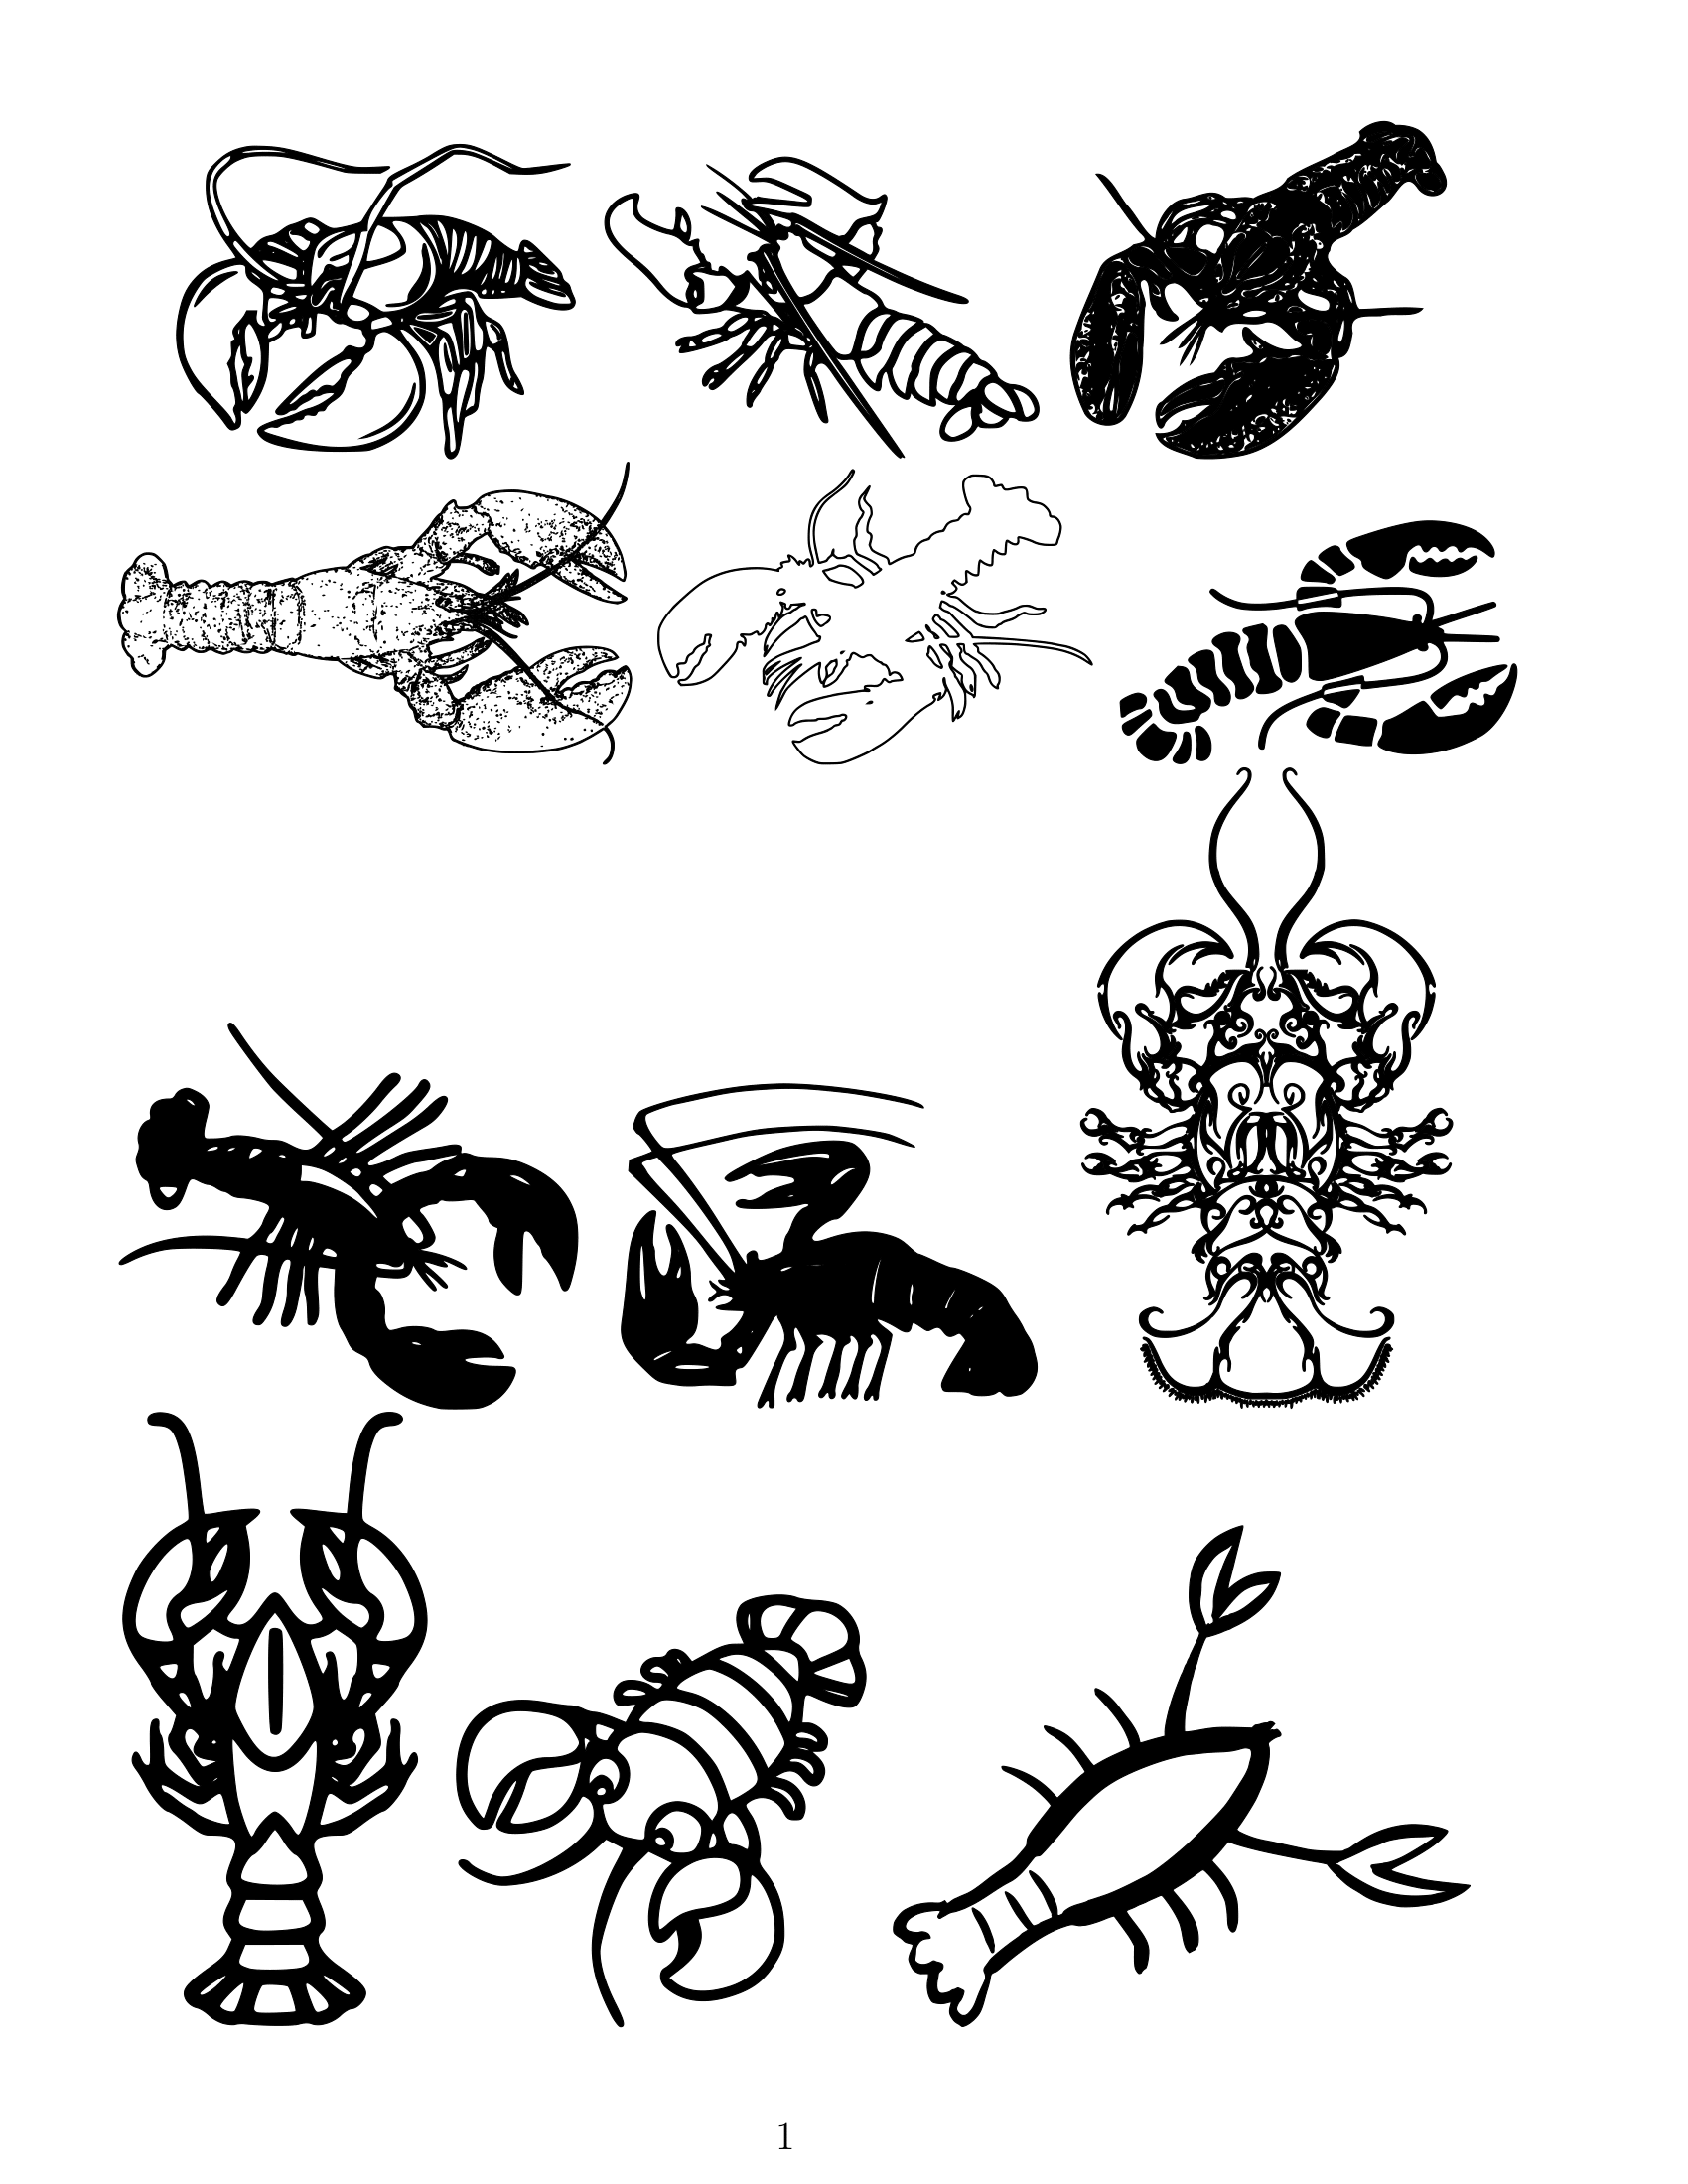
\includegraphics[width=1.2\linewidth]{lobsters_example-1.png}
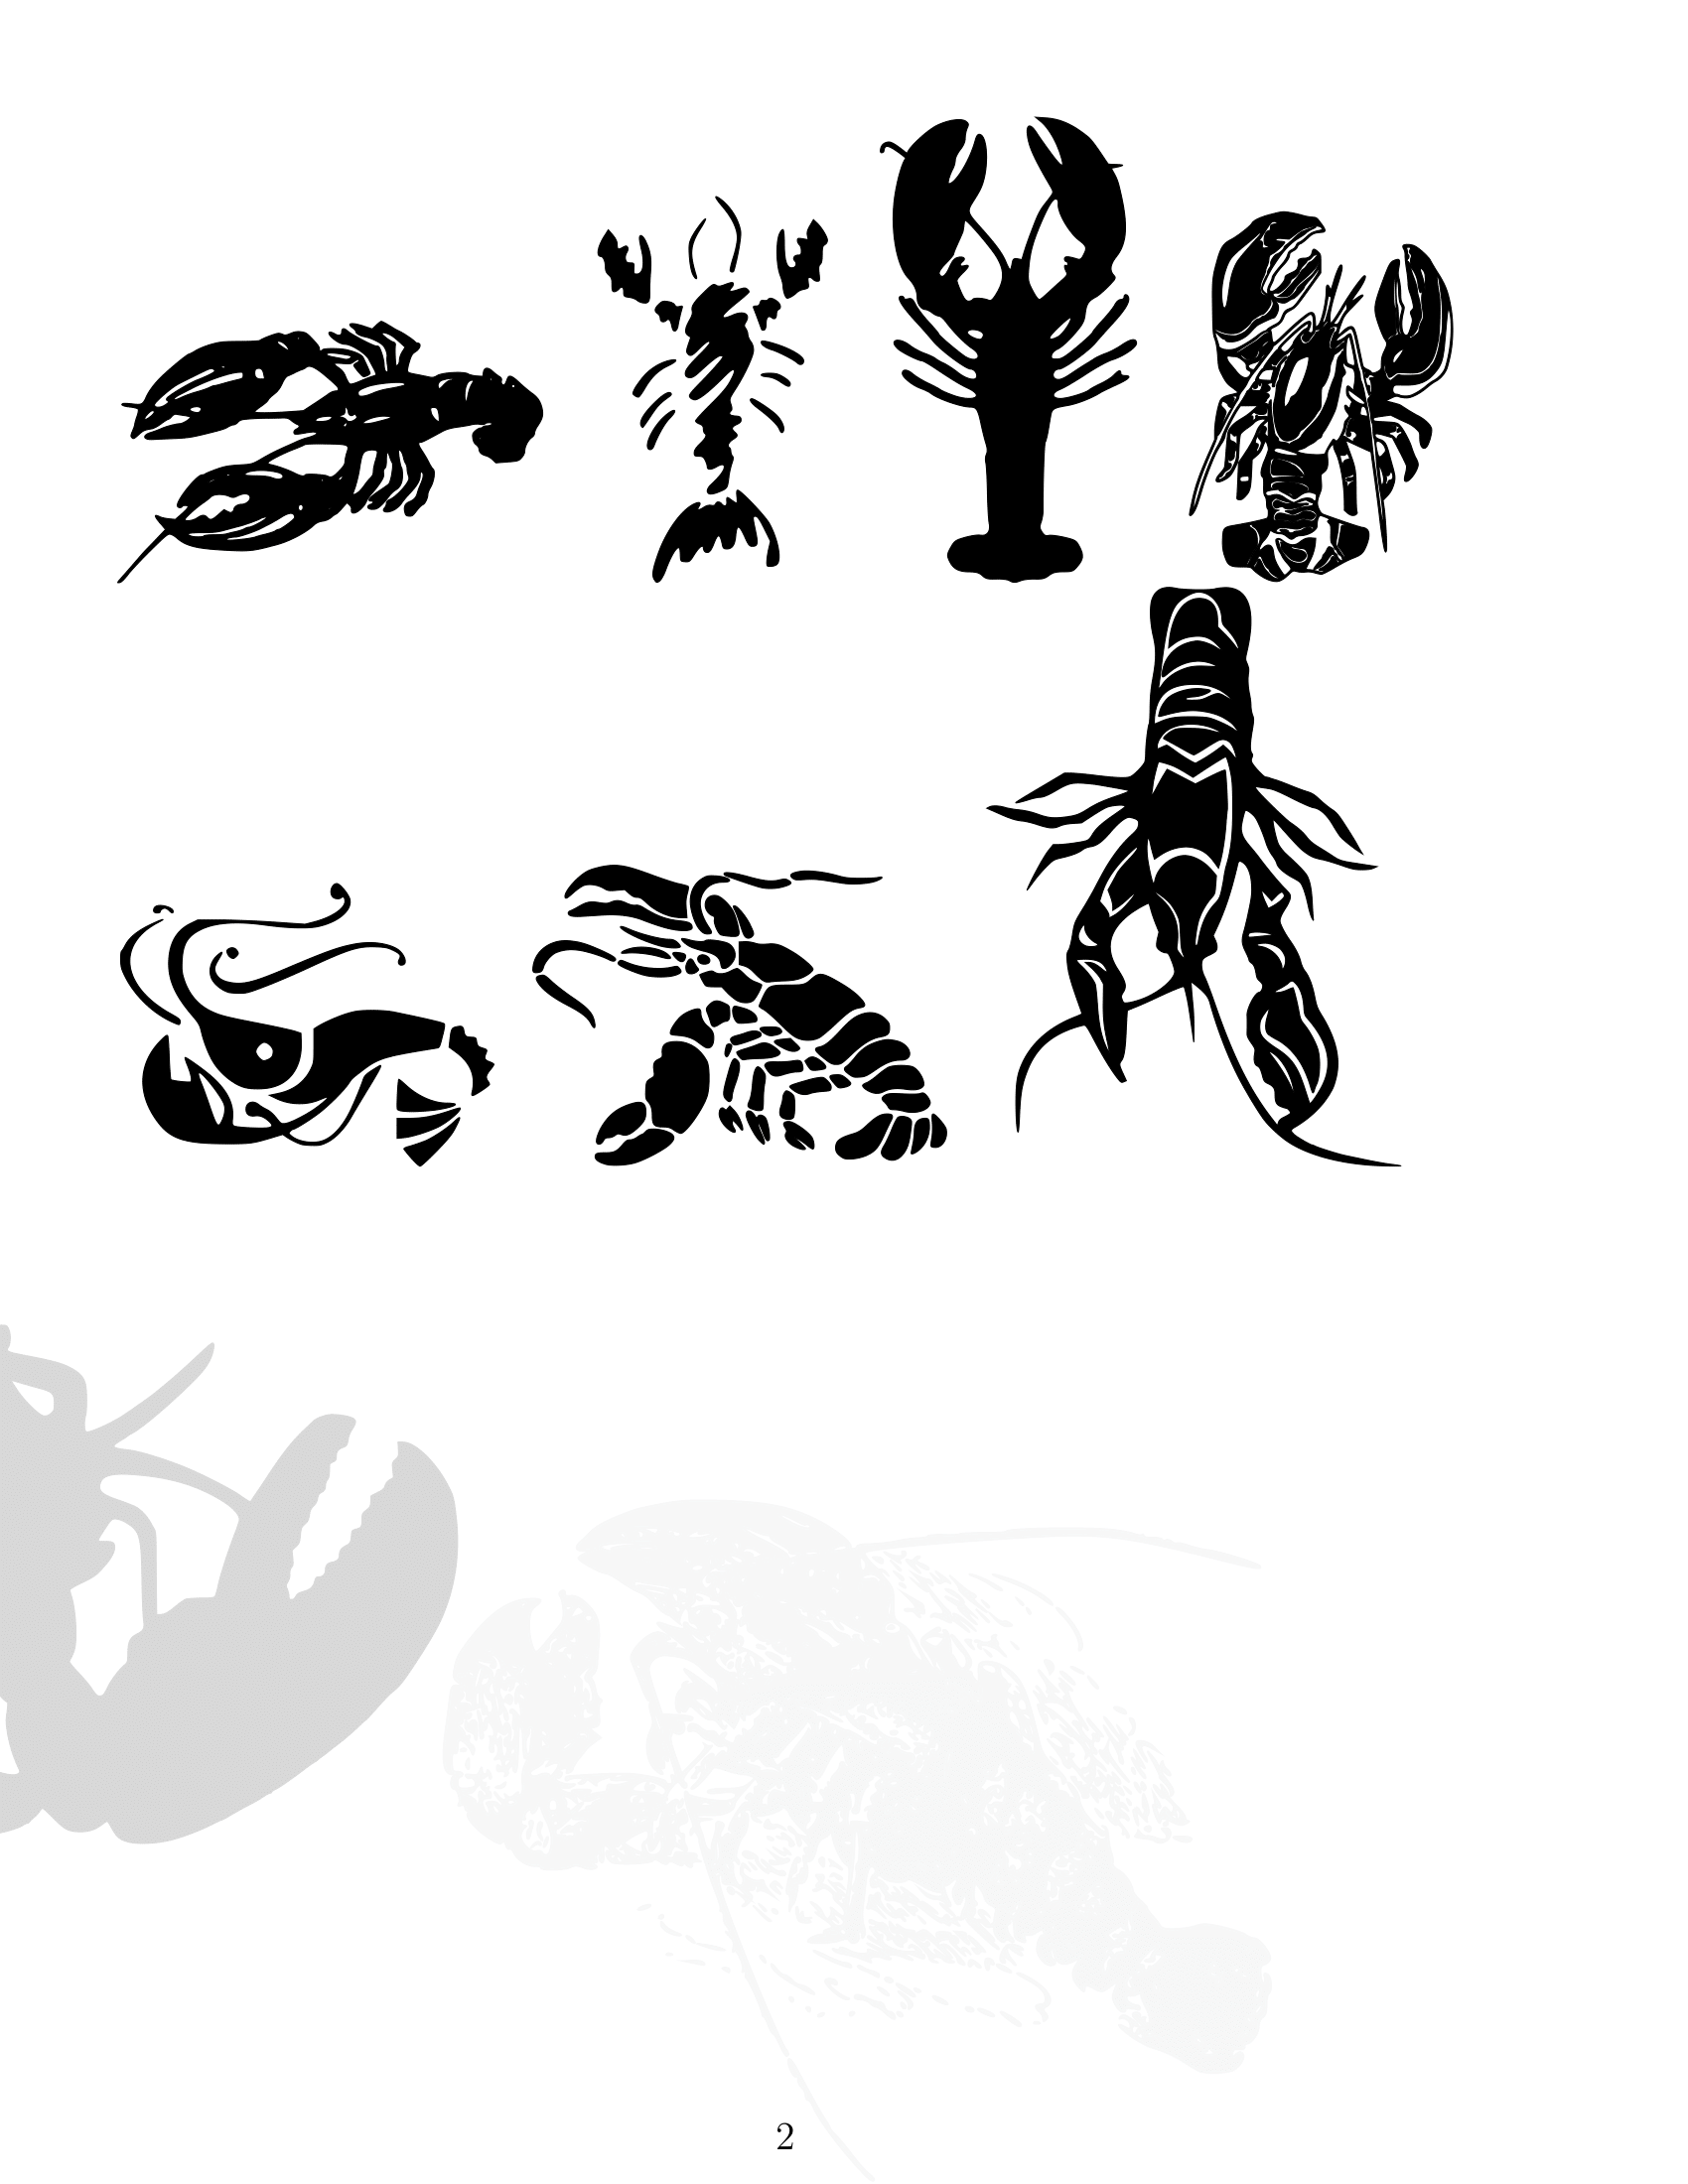
\includegraphics[width=1.2\linewidth]{lobsters_example-2.png}}{9.8}
\end{minipage}
&
\begin{minipage}[m]{0.55\textwidth}
\renewcommand\textminus{\mbox{-}}%<<<<<<<<<<<
\begin{lstlisting}[numberstyle=\zebra{orange!15}{red!15},numbers=left,basicstyle=\ttfamily\scriptsize]
\documentclass[14pt]{extreport}
\usepackage[left=1.5cm,right=3cm,top=1.5cm,
bottom=1.5cm,bindingoffset=0cm]{geometry}
\usepackage{loblib}
 
\begin{document}
\lob{1}     \lob{12}
\lob{2}     \lob{20}
\lob{3}     \lob{21}
\lob{4}     \lob{22}
\lob{5}     \lob{28}
\lob{6}     \lob{32}
\lob{7}     \lob{33}
\lob{8}     \lob{74}
\lob{9}     \lob{76}

\vspace*{2cm}
\hspace*{-2.8cm}
\definecolor{shadow}{rgb}{0.85,0.85,0.85}
\lob[rotate=-90,shadow,xscale=-1.2,yscale=1.2]{77}

\lobwatermark
\end{document}
\end{lstlisting}
LobLib documentation on \href{https://github.com/AnMnv/eBook}{GitHub} in \mybox[black]{LobLib-package} folder.\\ Origins of the package \href{https://github.com/bryce-evans/LobLib}{https://github.com/bryce-evans/LobLib}\\ However, to print lobsters put \mybox[red]{objects} folder and \mybox[red]{loblib.sty} from  the \mybox[black]{LobLib-package} folder into the same directory with your \mybox[brown]{.tex} file.
\end{minipage}
\end{tabular}
\end{table}
%#################### 9.9 ####################
\subsection{\hll{Watermark over \textbf{everything}}}
\begin{table}[h!]
\begin{tabular}{c | c}
\begin{minipage}[m]{0.4\textwidth}
\enum{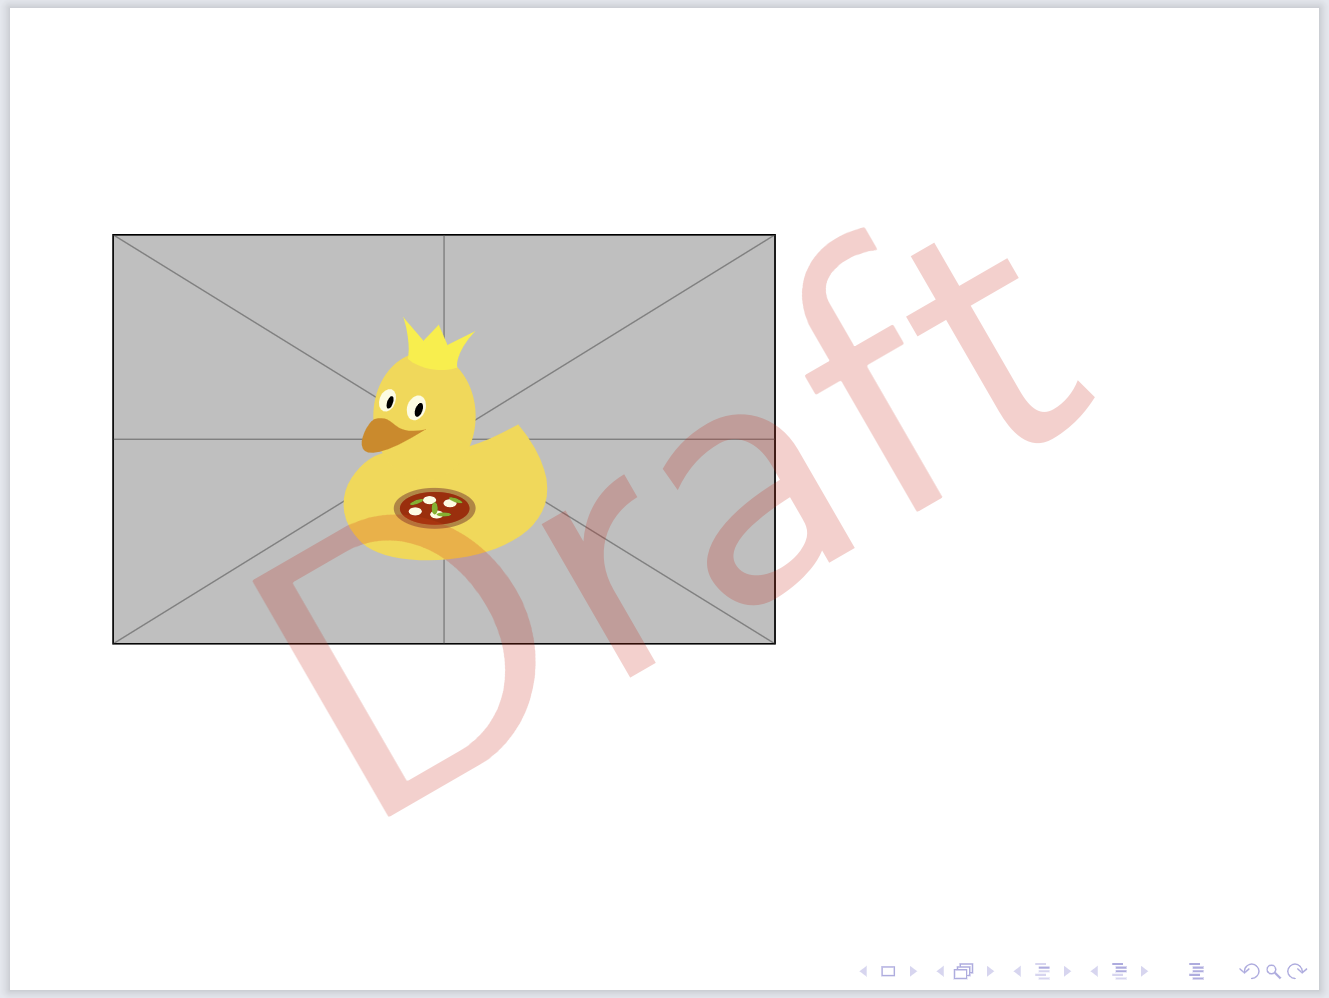
\includegraphics[width=1.\linewidth]{9.9.png}}{9.9}
\end{minipage}
&
\begin{minipage}[m]{0.55\textwidth}
\renewcommand\textminus{\mbox{-}}%<<<<<<<<<<<
\begin{lstlisting}[numberstyle=\zebra{orange!15}{red!15},numbers=left,basicstyle=\ttfamily\scriptsize]
\documentclass{beamer}

\usepackage{tikz}
\AddToHook{shipout/foreground}{
  \begin{tikzpicture}[remember picture,overlay]
    \node[red,rotate=30,scale=10,opacity=0.2] at (current page.center) {Draft}; 
  \end{tikzpicture}}

\begin{document}
\begin{frame}
\includegraphics{example-image-duck}
\end{frame}
\end{document}
\end{lstlisting}
\end{minipage}
\end{tabular}
\end{table}
%#################### 9.10 ####################
%#################### 9.11####################
%#################### 9.12 ####################
%#################### 9.13 ####################
